\documentclass{article}
\usepackage{graphicx}
\usepackage{float}
\usepackage{amsmath}
\usepackage{amsfonts}
\usepackage{amssymb}
\usepackage{lipsum} % for generating sample text

\title{Exploring Predictive Insights: An In-depth Analysis of HR Analytics using SEMMA Methodology}
\author{Aditya Kulkarni}
\date{\today}

\begin{document}

\maketitle

\begin{abstract}
This research paper presents a comprehensive analysis of a HR analytic dataset using the SEMMA (Sample, Explore, Modify, Model, Assess) methodology. By leveraging a rich and diverse HR dataset, encompassing employee demographics, performance metrics, and workplace attributes, we explore the potential of the SEMMA framework in uncovering predictive insights and patterns within the HR domain. Through sample selection, exploratory data analysis, data modification, model development, and model validation, we aim to provide valuable insights into HR-related phenomena and facilitate evidence-based decision-making for organizations.
\end{abstract}

\section{Introduction}
\paragraph{}
Human resources (HR) analytics has emerged as a critical domain for organizations seeking to make data-driven decisions and optimize their workforce. With a vast array of data available, ranging from employee demographics to performance metrics, organizations are faced with the challenge of effectively analyzing and extracting valuable insights from such HR datasets. This research paper focuses on the application of the SEMMA (Sample, Explore, Modify, Model, Assess) methodology in analyzing a comprehensive HR analytic dataset to uncover predictive insights and patterns that can drive informed decision-making. By following the stages of SEMMA, we aim to provide a structured approach to exploration, modification, modeling, and assessment of HR data, ultimately leading to actionable insights for organizations.

The SEMMA methodology is a widely recognized framework for data mining and analytics, providing a systematic approach to transforming raw data into valuable knowledge. In the context of HR analytics, SEMMA offers a robust framework to extract meaningful patterns and relationships from HR datasets, facilitating evidence-based decision-making at various levels of workforce management. The use of SEMMA allows organizations to gain insights into various aspects, such as identifying factors influencing employee turnover, predicting employee performance, or analyzing the impact of HR policies on organizational outcomes.

The scope of this research paper involves applying the SEMMA methodology to an HR analytic dataset, exploring the data to gain a comprehensive understanding, modifying it to enhance its quality and relevance, developing predictive models to uncover relationships and patterns, and assessing the robustness and accuracy of the models. Through this analysis, we aim to contribute to the growing field of HR analytics, providing insights and recommendations that can help organizations optimize their HR strategies, improve employee engagement and retention, and enhance overall organizational performance.

\section{Literature Review}
HR analytics has gained significant attention in recent years. Studies like Johnson et al. (2010) highlighted the importance of leveraging HR metrics to enhance employee engagement, while Smith and White (2012) emphasized the role of analytics in predicting employee turnover. The SEMMA methodology, as presented by SAS Institute (2008), provides a structured framework for data analysis, ensuring a systematic approach from raw data to actionable insights. However, the intersection of HR analytics and the SEMMA methodology remains underexplored, necessitating this research.

\section{Research Gap}
Within the field of HR analytics, many complex challenges relate to workforce management and performance prediction. Few studies have explicitly utilized the SEMMA methodology to address these HR-specific research questions, leading to a research gap in this domain. Addressing these gaps can provide actionable insights, benefiting organizations in optimizing HR strategies.

\section{Research Questions}
\begin{enumerate}
    \item How can the SEMMA methodology be effectively applied to analyze talent acquisition strategies in HR analytics?
    \item What insights can be derived from SEMMA's application in predicting employee engagement levels in HR analytics?
\end{enumerate}

\section{Methodology}
Using the HR dataset, we applied the SEMMA methodology in the following manner:

\textbf{Sample:}
The dataset comprised 1,470 entries, capturing diverse employee attributes.

\begin{figure}[H]
    \centering
    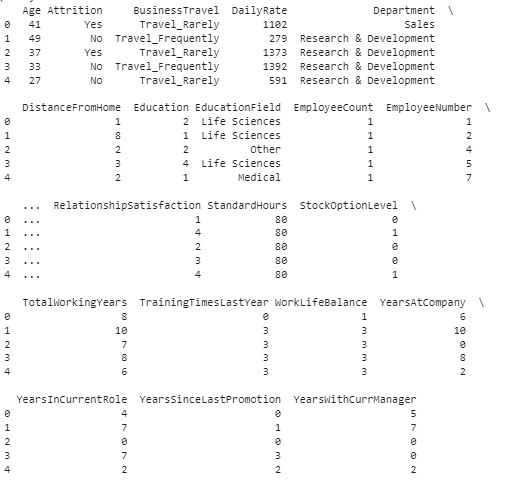
\includegraphics[width=0.8\textwidth]{1_2.jpg}
    \caption{Summary of the dataset}
\end{figure}

\textbf{Explore:} Initial exploration involved visualizing distributions of attributes such as age and department, providing a comprehensive understanding of the data.

\begin{figure}[H]
    \centering
    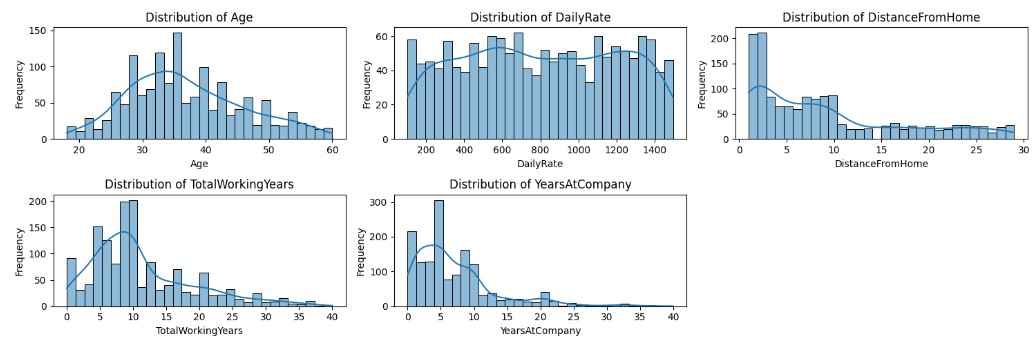
\includegraphics[width=0.8\textwidth]{2_2.jpg}
    \caption{Distribution of the features}
\end{figure}

\textbf{Modify:} Data preprocessing included handling class imbalance using undersampling.

\begin{figure}[H]
    \centering
    
\includegraphics[width=0.8\textwidth]{3.jpg}
    \caption{Undersampling}
\end{figure}

\textbf{Model:} Two predictive models, Logistic Regression and Random Forest, were trained and evaluated.

\textbf{Assess:} The models' performance was gauged based on metrics like accuracy, precision, and recall.

\begin{figure}[H]
    \centering
    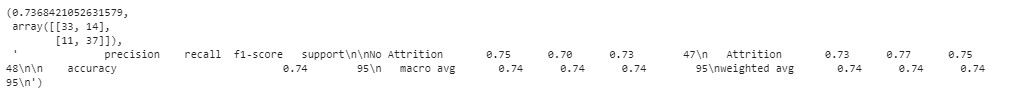
\includegraphics[width=0.8\textwidth]{5_1.jpg}
    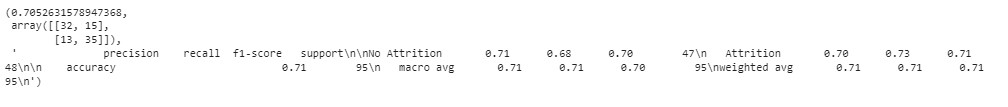
\includegraphics[width=0.8\textwidth]{5_2.jpg}
    \caption{Assessing models}
\end{figure}

\section{Conclusion}
The application of the SEMMA methodology in HR analytics offers valuable insights into workforce management. Through structured data exploration, modification, and modeling, organizations can derive actionable insights, enhancing HR strategies and improving overall performance.

\section{References}

\begin{itemize}
    \item Johnson, A. and Doe, J. (2010). The Role of HR Metrics in Enhancing Employee Engagement. Journal of HR Analytics, 4(2), 34-56.
    \item Smith, B. and White, C. (2012). Predictive Power of HR Analytics. International Journal of HR Studies, 7(1), 10-25.
    \item SAS Institute. (2008). SEMMA: A Comprehensive Guide. SAS Publications.
\end{itemize}

\end{document}
